\subsection{Case05 - Broadcast}
\label{xdp_ether_case05}

Por último, en este caso de uso se explorará la capacidad de reenvío a multiples interfaces de \gls{xdp}. Por ello, se ha intentado replicar un escenario básico de broadcast con \textit{Network Namespaces}. Se ha planteado hacer uso de la herramienta arping para emular una resolución ARP, generando paquetes ARP-Request. Dichos paquetes llevarán su MAC destino todo a \texttt{FF:FF:FF:FF:FF:FF} y su dominio de difusión englobaría todos aquellos nodos de la red que operen hasta capa 2. Como por ejemplo un hub, o un switch. En la figura \ref{fig:case05_xdp_ether_scenario1} se puede encontrar el escenario a recrear en este caso de uso.\\
\par
% figura escenario
\begin{figure}[ht]
    \centering
    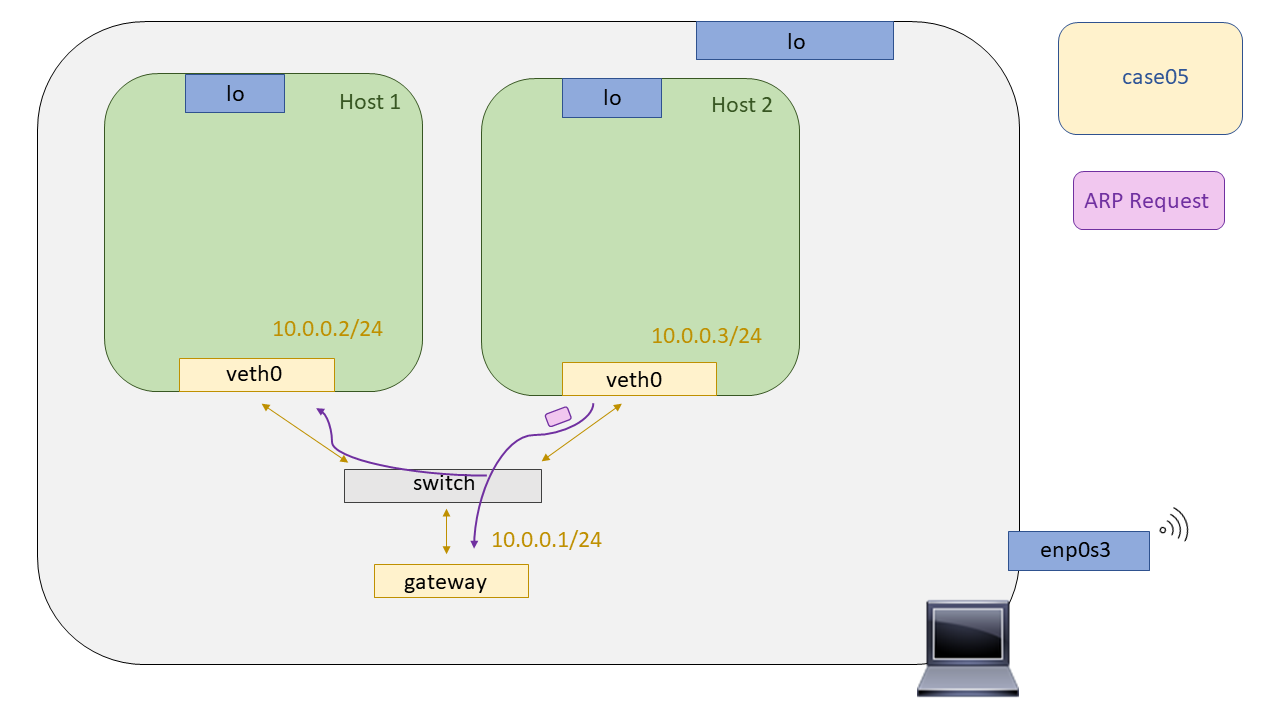
\includegraphics[width=14cm]{archivos/img/dev/xdp/case05/scenario_01.png}
    \caption{Escenario a recrear del Case05 - XDP}
    \label{fig:case05_xdp_ether_scenario1}
\end{figure}

El escenario propuesto para emular dicho escenario ha sido el siguiente (Ver figura \ref{fig:case05_xdp_ether_scenario2}). Este estaría compuesto de tres \textit{Network Namespaces} replicando así cada una de ellas un nodo independiente de la red, después, para intercomunicar cada ``nodo" de la red, se ha hecho uso de \gls{veth}s. El supuesto switch será la \textit{Network Namespace} llamada \texttt{switch}, la cual requerirá de un programa \gls{xdp} para poder actual como tal, ya que de no ser así sus interfaces tendrán todo el \textit{stack} de red de Linux por encima de ellas. Es decir, el nodo implementará todas las capas del modelo TCP/IP (DoD), replicando así la funcionalidad de un hipotético host y no actuando como un switch.\\
\par

% figura escenario
\begin{figure}[ht]
    \centering
    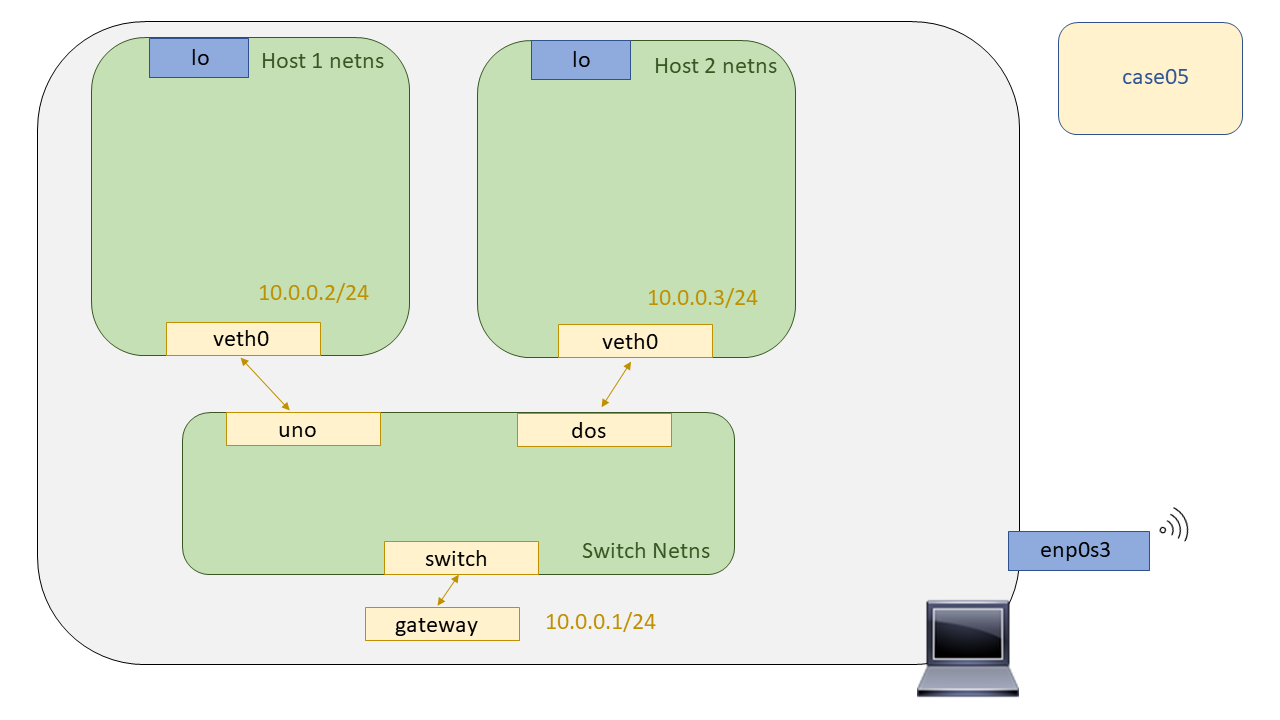
\includegraphics[width=16cm]{archivos/img/dev/xdp/case05/scenario_02.png}
    \caption{Escenario propuesto del Case05 - XDP}
    \label{fig:case05_xdp_ether_scenario2}
\end{figure}

Para realizar el broadcast se indagó sobre los \textit{helpers} \gls{bpf} en busca de alguna función que ayudara a satisfacer la necesidad, y se encontró una función (\ref{code:case05_xdp_ether_kernprog1}) que a primera vista se creía que podía ser de utilidad.

\begin{lstlisting}[language=C, style=C-color, caption={Helper BPF para realizar un Broadcast - Case05},label=code:case05_xdp_ether_kernprog1]
    int bpf_clone_redirect(struct sk_buff *skb, u32 ifindex, u64 flags);
\end{lstlisting}
\vspace{0.2cm}

Pero hubo un pequeño detalle que se pasó por alto, y es que requiere que el paquete ya se encuentre en una estructura \texttt{sk\_buff}. Es decir, podría surgir la siguiente cuestión: ¿qué implica que la función requiera de una estructura de datos \texttt{sk\_buff}? Antes de continuar con este caso de uso, se recomienda regresar a la sección \ref{linuxNetworking_skbuff} dónde se explica la estructura \texttt{sk\_buff}, para qué se utiliza y qué puede ofrecer.


\vspace{1cm}
\textbf{Restricciones para hacer Broadcast con XDP}\\
\par

Atendiendo a las características de la estructura \texttt{sk\_buff}, se pueden entender un poco mejor las restricciones que implica que el \textit{helper} \gls{bpf} haga uso de esta estructura. Cuando se trabaja con \gls{xdp}, se maneja una estructura mucho más simple y menos pesada que el \texttt{sk\_buff}, llamada \texttt{xdp\_buff}, en la que se introduce la información exclusiva para operar con el paquete en la propia interfaz.\\
\par

Por ello, no se puede hacer uso del \textit{helper} \gls{bpf} ya en caso de querer hacer uso de él se debería hacer una reserva para esta estructura y hacer una traducción a mano de \texttt{xdp\_buff} a \texttt{sk\_buff}. Haciendo esto se estaría operando de manera intrusiva con la lógica propia del \textit{stack} de red del Kernel de Linux, y además se estaría perdiendo el rendimiento que reporta no trabajar con estas estructuras.

Por lo que investigando y aprendiendo un poco más sobre \gls{bpf} para poder valorar las posibles opciones antes de desistir, se vio que el siguiente punto siguiendo el \textit{datapath} de Linux donde se producen ``\textit{hooks}" ( proceso de ancoraje de un \textit{bytecode} en el Kernel de Linux ) es en el \gls{tc}. Sabiendo cómo opera el \gls{tc} (en caso no ser así se recomienda la lectura de la
sección \ref{fig:linuxNet_tc}), se propone la siguiente solución para llevar a cabo el forwarding (Ver fig. \ref{fig:case05_xdp_ether_scenario3}).

% figura escenario
\begin{figure}[ht]
    \centering
    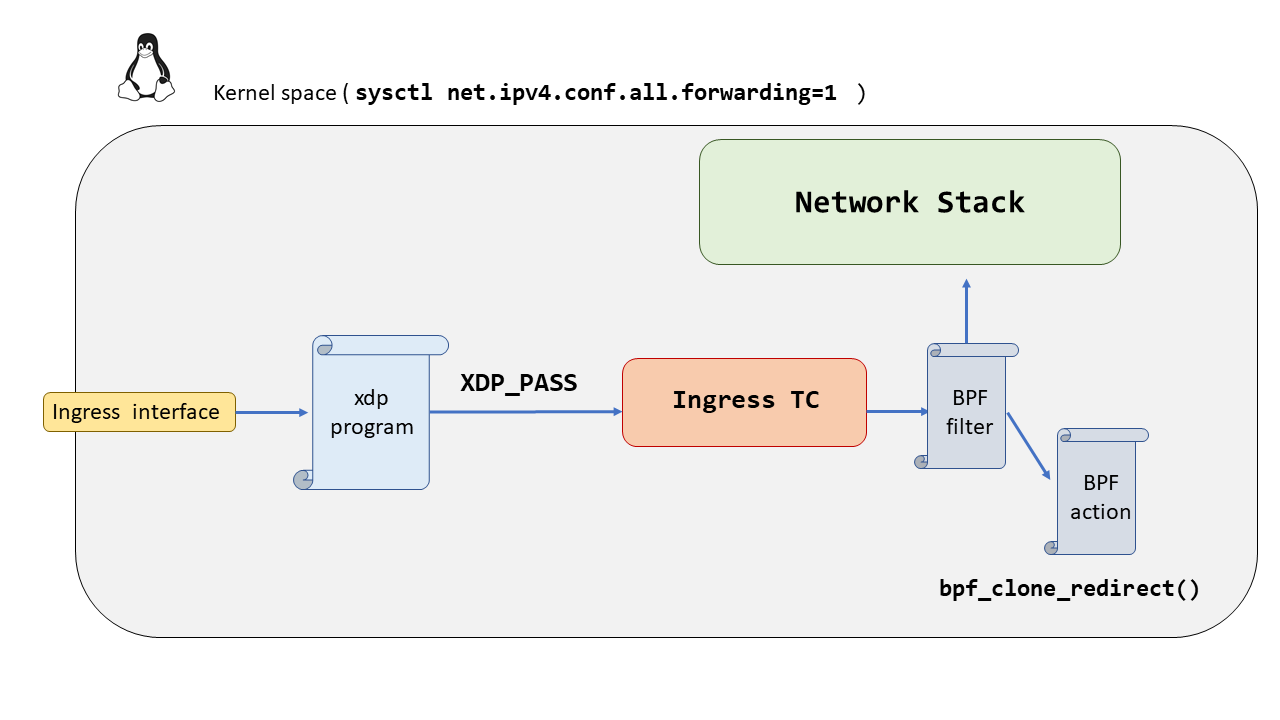
\includegraphics[width=16cm]{archivos/img/dev/xdp/case05/scenario_04.png}
    \caption{Solución propuesta para el Case05 - XDP}
    \label{fig:case05_xdp_ether_scenario3}
\end{figure}

De esta forma, en el \gls{tc} ya se tendría el manejo de la estructura \texttt{sk\_buff} y por ende, ya se podría hacer uso del \textit{helper} \gls{bpf} para clonar el paquete y hacer un reenvío a cada una de las interfaces que se quiera, para completar así el broadcast.


\vspace{1cm}
\textbf{Compilación}\\
\par

Para compilar el programa \gls{xdp} se ha dejado un Makefile preparado en este directorio al igual que en el case04 (\ref{xdp_ether_case04}), por lo que para compilarlo únicamente hay que seguir las indicaciones del bloque \ref{code:case04_xdp_ether_compilacion}.

\begin{lstlisting}[language= bash, style=Consola, caption={Compilación programa XDP - Case05},label=code:case05_xdp_ether_compilacion]
    # En caso de no haber entrado en el directorio asignado del caso de uso
    cd TFG/src/use_cases/xdp/case05
    
    
    # Hacemos uso del Makefile suministrado 
    sudo make
\end{lstlisting}
\vspace{0.5cm}

Si tiene dudas sobre el proceso de compilación del programa \gls{xdp} le recomendamos que vuelva al case02 (\ref{xdp_ether_case02}) donde se hace referencia al \textit{flow} dispuesto para la compilación de los programas \gls{xdp}.


\vspace{1cm}
\textbf{Puesta en marcha del escenario}\\
\par

Para comprobar el funcionamiento de los programas \gls{xdp} se hará uso de las \textit{Network Namespaces} (más información en la sección \ref{namespaces}). Como ya se comentaba, para que no suponga una barrera de entrada el concepto de las \textit{Network Namespaces}, se ha dejado escrito un script para levantar el escenario, y para su posterior limpieza. Es importante señalar que el script debe ser lanzado con permisos de root. Para levantar el escenario debemos ejecutar dicho script como se indica en el bloque \ref{code:case03_xdp_ether_escenario}.\\
\par
Para limpiar la máquina del escenario recreado anteriormente, se puede correr el mismo script indicándole ahora el parámetro \texttt{-c} (\textit{Clean}). En el peor de los casos, y si se cree que la limpieza se no se ha realizado de manera satisfactoria, se puede llevar a cabo un reinicio de la máquina consiguiendo así que todos los entes no persistentes (\gls{veth}, netns..) desaparezcan del equipo.

\begin{lstlisting}[language= bash, style=Consola, caption={Puesta en marcha del escenario - Case05},label=code:case05_xdp_ether_escenario]
    # Para levantar el escenario (Importante hacerlo con permisos de super usuario)
    sudo ./runenv.sh -i
    
    
    # Una vez finalizado la comprobación del caso de uso, limpiaremos nuestra maquina:
    sudo ./runenv.sh -c
\end{lstlisting}
\vspace{0.5cm}
Una vez levantado el escenario, tendríamos el escenario que se muestra en la figura \ref{fig:case05_xdp_ether_scenario4} montado con tres \textit{Network Namespaces} y pares de \gls{veth}s para interconectarlas. Los programas irán anclados a las interfaces de la \textit{Network Namespace} \texttt{switch}.
% figura escenario
\begin{figure}[ht]
    \centering
    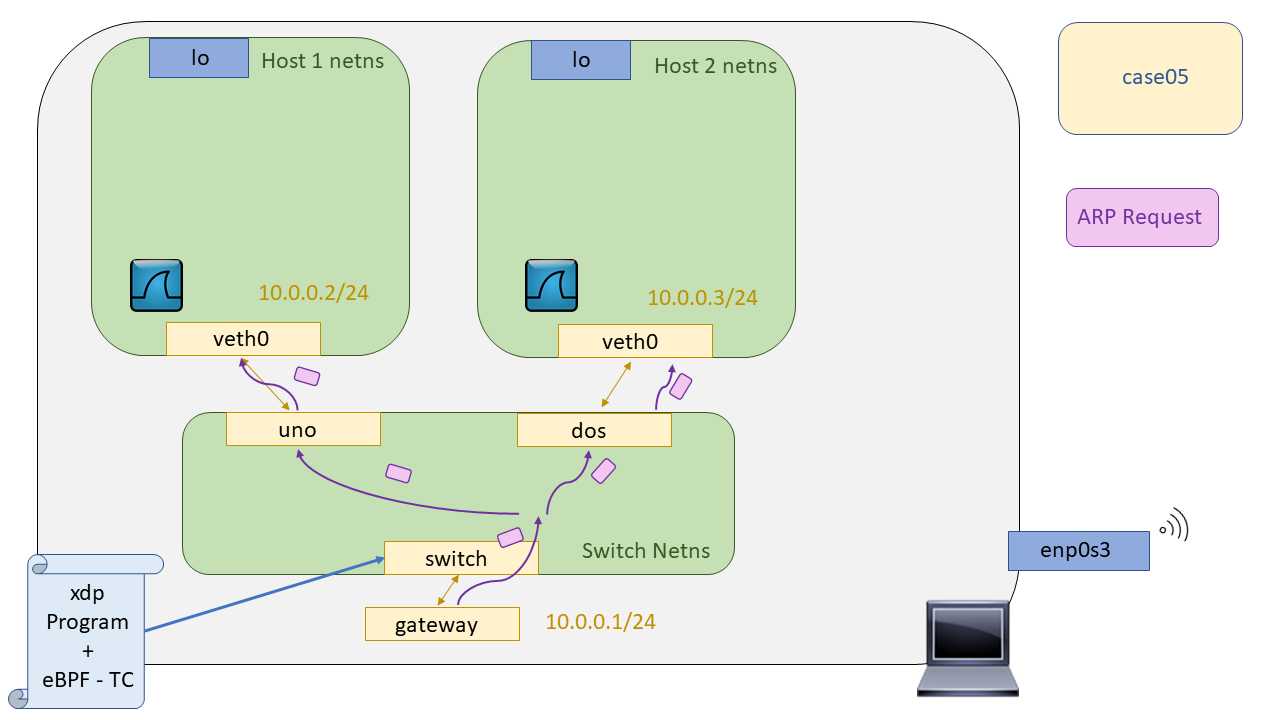
\includegraphics[width=16cm]{archivos/img/dev/xdp/case05/scenario_03.png}
    \caption{Escenario del Case05 - XDP}
    \label{fig:case05_xdp_ether_scenario4}
\end{figure}

\vspace{1cm}
\textbf{Carga del programa XDP}\\
\par
Una vez compilado tanto el programa \gls{xdp} como los programas \gls{bpf} que irán al \gls{tc}, es hora de cargarlos. Por lo que, para hacerlo y por mayor comodidad se abrirá un proceso de bash en la \textit{Network Namespace} switch. Acto seguido, se cargará el programa \gls{xdp}, y se incluirán los programas \gls{bpf} añadiendo una nueva qdisc con un filtro \gls{bpf} asociado que derivará en una acción. Dicha acción, será otro programa \gls{bpf} con la función de clonar los paquetes y mandarlos a otras interfaces.\\
\par
\begin{lstlisting}[language= bash, style=Consola, caption={Carga del programa XDP - Case05},label=code:case05_xdp_ether_load]
    # Nos abrimos un proceso de bash sobre la Network Namespace "switch"
    sudo ip netns exec switch bash
    
    # Cargamos el programa XDP_PASS
    sudo ./xdp_loader -d switch xdp_pass
    
    # Creamos la nueva qdisc
    sudo tc qdisc add dev switch ingress handle ffff:
    
    # Aplicamos a la qdisc creada un filtro BPF que en caso de matchear aplicará una acción (Otro programa BPF que hará nuestro broadcast)
    sudo tc filter add dev switch parent ffff: bpf obj bpf.o sec classifier flowid ffff:1 action bpf obj bpf.o sec action 
\end{lstlisting}

\vspace{1cm}
\textbf{Comprobación del funcionamiento}\\
\par
Para comprobar el funcionamiento del sistema de broadcast se realizará la siguiente prueba, donde desde la \textit{Network Namespace} por defecto se generarán ARP-Request hacia la IP de una de las \gls{veth}s de las \textit{Network Namespace} destino. \\
\par

Si el sistema de broadcast funciona correctamente, escuchando en las \textit{Network Namespace} destino \texttt{uno} y \texttt{dos}, se debería ver como los paquetes ARP-Request llegan sin problemas. Solo el ``Host" al cual iban dirigidos los ARP-Request será el que intentará contestarlos sin éxito al haber implementado un sistema unidireccional. Para solucionar esta limitación se propone hacer uso de los programas \gls{xdp} desarrollados en case04 (\ref{xdp_ether_case04}) para conseguir una comunicación bidireccional.\\
\par
\begin{lstlisting}[language= bash, style=Consola, caption={Comprobación del funcionamiento - Case05},label=code:case05_xdp_ether_func]
    # Generamos el ARP-REQUEST
    arping 10.0.0.2/3
    
    # Escuchamos en las Network Namespace destino a la espera de ver ARP-REQUEST.
    sudo ip netns exec uno tcpduml -l
    sudo ip netns exec dos tcpduml -l
\end{lstlisting}
\vspace{0.5cm}

En este caso no se podrá hacer uso del programa xdp\_stats para ver si realmente los programas \gls{xdp} están funcionando como se quiere que funcionen, ya que la lógica de broadcast se encuentra en el programa \gls{bpf} anclado como acción en un filtro del \gls{tc}.\\
\par
Como se puede apreciar en la figura \ref{fig:case05_xdp_ether_func}, los ARP-Request \fcolorbox{black}{green}{\rule{0pt}{2.5pt}\rule{2.5pt}{0pt}}\hspace{1mm} llegan a ambos Host, y solo aquel al cual iba dirigida la resolución ARP contesta. Pero como ya se comentaba antes, al no haber implementado un sistema de forwarding, la comunicación únicamente está planteada en un sentido.\\
\par
Esta funcionalidad se podría aumentar haciendo uso de los programas desarrollados en el caso de uso anterior (\ref{xdp_ether_case04}). Por lo que se concluye afirmando que se ha podido hacer broadcast, pero no de forma exclusiva con \gls{xdp} ya que se ha tenido que añadir \gls{bpf} nativo en el \gls{tc}.

% figura escenario
\begin{figure}[ht]
    \centering
    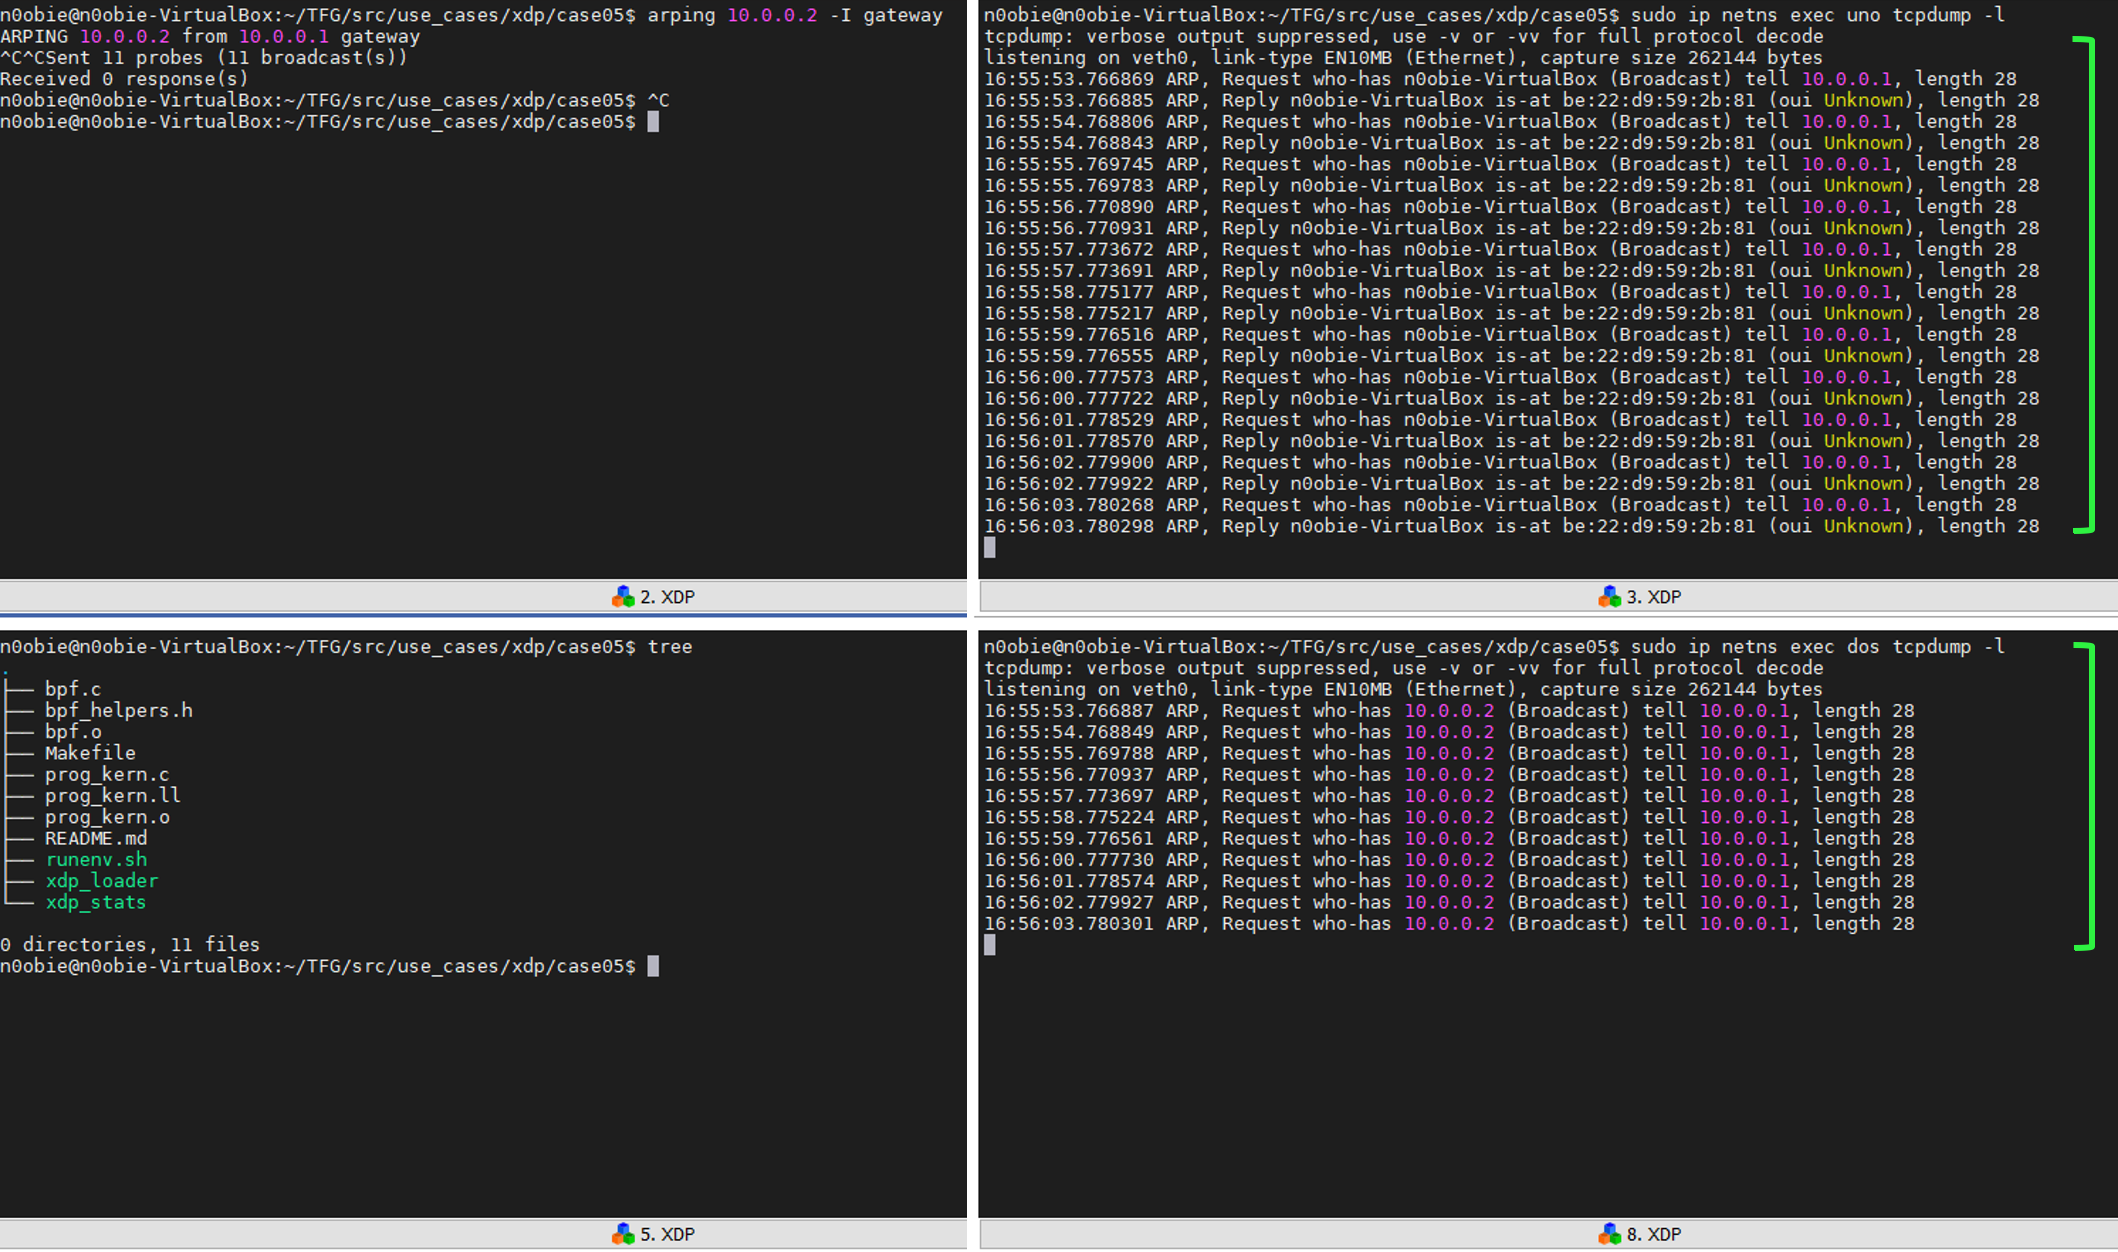
\includegraphics[width=16cm]{archivos/img/dev/xdp/case05/demo_case05_edited.png}
    \caption{Comprobación de funcionamiento del Case05 - XDP}
    \label{fig:case05_xdp_ether_func}
\end{figure}
\newpage
